\documentclass{article}
\usepackage[margin=1in]{geometry}
\usepackage{physics}
\usepackage{graphicx}
\usepackage{caption}
\usepackage{amsmath}
\usepackage{bm}
\usepackage{authblk}
\usepackage{empheq}
\usepackage{amsfonts}
\usepackage{esint}
\usepackage[makeroom]{cancel}
\usepackage{dsfont}
\usepackage{centernot}
\usepackage{mathtools}
\usepackage{bigints}
\usepackage{amsthm}
\theoremstyle{definition}
\newtheorem{defn}{Definition}[section]
\newtheorem{prop}{Proposition}[section]
\newtheorem{rmk}{Remark}[section]
\newtheorem{thm}{Theorem}[section]
\newtheorem{exmp}{Example}[section]
\newtheorem{prob}{Problem}[section]
\newtheorem{sln}{Solution}[section]
\newtheorem*{prob*}{Problem}
\newtheorem{exer}{Exercise}[section]
\newtheorem*{exer*}{Exercise}
\newtheorem*{sln*}{Solution}
\usepackage{empheq}
\usepackage{hyperref}
\usepackage{tensor}
\usepackage{xcolor}
\hypersetup{
	colorlinks,
	linkcolor={black!50!black},
	citecolor={blue!50!black},
	urlcolor={blue!80!black}
}


\newcommand*\widefbox[1]{\fbox{\hspace{2em}#1\hspace{2em}}}

\newcommand{\p}{\partial}
\newcommand{\R}{\mathbb{R}}
\newcommand{\C}{\mathbb{C}}
\newcommand{\lag}{\mathcal{L}}
\newcommand{\nn}{\nonumber}
\newcommand{\ham}{\mathcal{H}}
\newcommand{\M}{\mathcal{M}}
\newcommand{\I}{\mathcal{I}}
\newcommand{\K}{\mathcal{K}}
\newcommand{\F}{\mathcal{F}}
\newcommand{\w}{\omega}
\newcommand{\lam}{\lambda}
\newcommand{\al}{\alpha}
\newcommand{\be}{\beta}
\newcommand{\x}{\xi}

\newcommand{\G}{\mathcal{G}}

\newcommand{\f}[2]{\frac{#1}{#2}}

\newcommand{\ift}{\infty}

\newcommand{\lp}{\left(}
\newcommand{\rp}{\right)}

\newcommand{\lb}{\left[}
\newcommand{\rb}{\right]}

\newcommand{\lc}{\left\{}
\newcommand{\rc}{\right\}}


\newcommand{\V}{\mathbf{V}}
\newcommand{\U}{\mathcal{U}}
\newcommand{\Id}{\mathcal{I}}
\newcommand{\D}{\mathcal{D}}
\newcommand{\Z}{\mathcal{Z}}

%\setcounter{chapter}{-1}


%\makeatletter
%\renewcommand{\@chapapp}{Part}
%\renewcommand\thechapter{$\bf{\ket{\arabic{chapter}}}$}
%\renewcommand\thesection{$\bf{\ket{\arabic{section}}}$}
%\renewcommand\thesubsection{$\bf{\ket{\arabic{subsection}}}$}
%\renewcommand\thesubsubsection{$\bf{\ket{\arabic{subsubsection}}}$}
%\makeatother



\usepackage{subfig}
\usepackage{listings}
\captionsetup[lstlisting]{margin=0cm,format=hang,font=small,format=plain,labelfont={bf,up},textfont={it}}
\renewcommand*{\lstlistingname}{Code \textcolor{violet}{\textsl{Mathematica}}}
\definecolor{gris245}{RGB}{245,245,245}
\definecolor{olive}{RGB}{50,140,50}
\definecolor{brun}{RGB}{175,100,80}
\lstset{
	tabsize=4,
	frame=single,
	language=mathematica,
	basicstyle=\scriptsize\ttfamily,
	keywordstyle=\color{black},
	backgroundcolor=\color{gris245},
	commentstyle=\color{gray},
	showstringspaces=false,
	emph={
		r1,
		r2,
		epsilon,epsilon_,
		Newton,Newton_
	},emphstyle={\color{olive}},
	emph={[2]
		L,
		CouleurCourbe,
		PotentielEffectif,
		IdCourbe,
		Courbe
	},emphstyle={[2]\color{blue}},
	emph={[3]r,r_,n,n_},emphstyle={[3]\color{magenta}}
}


\begin{document}
\begin{center}
	\huge{Ideas \#4: Bringing in oscillatory integrals}\\
	$\,$\\
	\normalsize{\today}\\
	\normalsize{Huan Bui}
\end{center}
\begin{figure}[!htb]
	\centering
	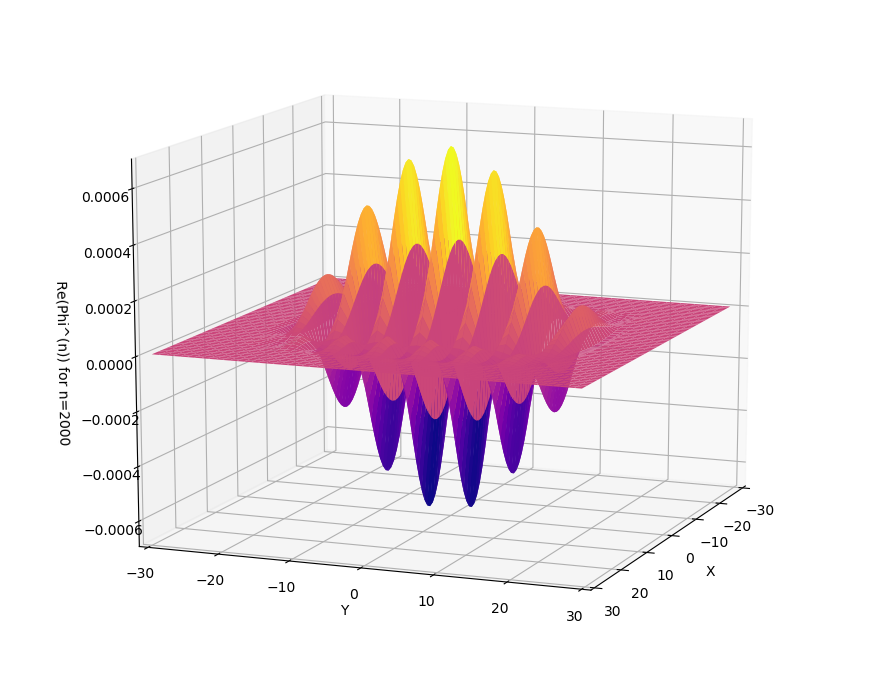
\includegraphics[scale=0.4]{conv_1}
	\caption{The real part of the convolution powers ($n=2000$) of the first $\phi$ in the $\mathbb{Z}^d$ paper. In this notebook I am interested in finding a new $\phi$ whose attractor involves an oscillatory integral and compute its convolution powers.}
\end{figure}


The goal here is to find a $\phi: \mathbb{Z}^2 \to \C$ such that the attractor of its convolution powers involves an oscillatory integral. Note that we don't know whether the attractor exists or not, or in which sense it exists if it does. The goal here is different from those of last semester, where we focused primarily on the parameterization 
\begin{align}
\xi \to t^{-E} s
\end{align} 
in order to absorb the leading $t$ in the integrand of
\begin{align}
\int e^{-itP(\xi) - ix\cdot \xi}\,d\xi \to  \int e^{-ix\cdot t^{E}s}\,\abs{J}ds 
\end{align}
into $P(\xi)$ via $tP(\xi) = P(t^E \xi) = P(s)$. When requiring $s$ be in a (compact) space such that $P(s) = 1$, we simplified the integral considerably but also introduced a Jacobian due to the $\xi \leftrightarrow s$ transformation. We spent some time worrying about how to deal with actually evaluating the new volume (and eventually the integral) due to the scaling factor. I suggested an iterative way to evaluate the new volume, which guarantees a finite answer up to some scaling factor. Evan suggested a way to express the Jacobian entirely in terms of $P(\xi)$ and its powers. While we haven't evaluated the integral with the $e^{-ix\cdot t^Es}$ part of the integrand, I think we have at least some sense of what things can look like once we try. 

\newpage

The problem I think we are interested in now is actually seeing how the convolution powers of a $\phi$ behave when the attractor involves an oscillatory integral. This means now we wish to construct a $\phi$ (in $\mathbb{Z}^2$ for now) such that the attractor we get is something like the integral above where there's a factor of $i$ multiplying $P(\xi)$, which makes the integral oscillatory. \\

To this end I wrote a little program in Python which can calculate and plot convolution powers. Under certain constraints it seems to work pretty well (as you can tell from Figure 1). I will use it to look at $\phi^{(n)}$ once one is found. \\

To find a $\phi(\xi)$ I will rely on one of the examples in the $\mathbb{Z}^d$ paper where 
\begin{align}
E = \begin{pmatrix}
1/2 & 0\\
0 & 1/4
\end{pmatrix}.
\end{align}


First we recall (very roughly) how to get from $\phi(\xi)$ to the attractor of its convolution powers. Starting with a $\phi: \mathbb{Z}^d \to C$, we know that the Fourier transform of convolution powers is powers of the Fourier transform. So
\begin{align}
\phi^{(n)}(x) = \f{1}{(2\pi)^d}\int_{\mathbb{T}^d} e^{-ix\cdot \xi} [\hat{\phi}(\xi)]^n\,d\xi
\end{align} 
where $x\in \mathbb{Z}^d$, and $\mathbb{T}^d = (-\pi ,\pi ]^d$ is roughly speaking the Fourier space. Next, we are interested in the local behavior of $\hat{\phi}$, to which end we write $\hat{\phi} = \exp\lp \log(\hat{\phi}) \rp$ and define $\Gamma_{\xi_0}: \mathcal{U}\subseteq\mathbb{R}^d \to \C$ by
\begin{align}
\Gamma_{\xi_0} = \log\lp \f{\hat{\phi}(\xi+\xi_0)}{\hat{\phi}(\xi_0)} \rp
\end{align}
where $\xi_0 \in \Omega(\phi) = \lc \xi \in \mathbb{T}^d : \abs{\hat{\phi}(\xi)} = 1 \rc$, $\log$ is the principal branch of logarithm. Because $\hat{\phi}$ is smooth, $\Gamma_{\xi_0} \in C^\infty(\mathcal{U})$ and so we can use Taylor's theorem to approximate $\Gamma_{\xi_0}$ near 0.\\

Here, since we're no longer interested in the case where the Taylor expansion yields a positive homogeneous polynomial, we will diverge from the paper's discussion of $\xi_0$ being of positive homogeneous type. Rather, we'll just look at the Taylor's expansion for $\Gamma_{\xi_0}$ and see how to make $P_{\xi_0}(\xi)$ carry an $i$. The Taylor's expansion of $\Gamma_{\xi_0}(\xi)$ around $0 \in \mathbb{R}^2$ (since we're only interested in the $\mathbb{Z}^2$ for now) is given by
\begin{align}
\Gamma_{(\eta_0,\zeta_0)} \approx \cancel{\Gamma_{\xi_0}(0)} + \Gamma_{\eta_0}(0,0)()
\end{align} 




\newpage

\section*{Python code for calculating/approximating convolution powers}

Note that the convolution power procedure I'm using the generate the figure is the ``fast\_convolve(.)'' function. It is much faster than the standard convolve(.) function because I make it bound the support of $\phi^{(n)}$ when the support reaches some (variable) critical value. I checked and the two procedures seem to agree very well up to $n=100$, at which point the standard procedure stops working (at least for this particular $\phi$). I'll try to improve this little program, but so far it seems to work fine up to $n=10,000$, under some constraints. \\

\textbf{Here's the code.} As you can see it is quite short. This took me about 1-2 hours to write. 
\begin{lstlisting}
import numpy as np
import matplotlib.pyplot as plt
from scipy import signal
from matplotlib import cm, colors
from mpl_toolkits.mplot3d.axes3d import Axes3D
import operator
import time



def convolve(n_times):
Phi = np.array([[0, 0, 0, 0, 0],
[0, complex(0,-1)*(np.sqrt(3)-1), complex(2,-2), complex(0,-1)*(np.sqrt(3)-1), 0],
[-2, 5+np.sqrt(3), 8, 5+np.sqrt(3), -2],
[0, complex(0, 1)*(np.sqrt(3)-1), complex(2,+2), complex(0, 1)*(np.sqrt(3)-1), 0],
[0, 0, 0, 0, 0]])

Phi = Phi/(22+2*np.sqrt(3))
conv_power = np.copy(Phi)

i=0
while i < n_times:
conv_power = signal.convolve2d(Phi, conv_power, 'full')
i += 1

return conv_power



def fast_convolve(n_times, support_bound):
Phi = np.array([[0, 0, 0, 0, 0],
[0, complex(0,-1)*(np.sqrt(3)-1), complex(2,-2), complex(0,-1)*(np.sqrt(3)-1), 0],
[-2, 5+np.sqrt(3), 8, 5+np.sqrt(3), -2],
[0, complex(0, 1)*(np.sqrt(3)-1), complex(2,+2), complex(0, 1)*(np.sqrt(3)-1), 0],
[0, 0, 0, 0, 0]])

Phi = Phi/(22+2*np.sqrt(3))    
conv_power = np.copy(Phi)

i=0
while i < n_times:
conv_power = signal.convolve2d(Phi, conv_power, 'full')
dim_f = np.shape(conv_power)
if dim_f[0] > support_bound or dim_f[0] > support_bound:
conv_power = cropND(conv_power,(40,40))
i += 1

return conv_power


def cropND(img, bounding):
if bounding[0] <= np.shape(img)[0] and bounding[1] <= np.shape(img)[1]:
start = tuple(map(lambda a, da: a//2-da//2, img.shape, bounding))
end = tuple(map(operator.add, start, bounding))
slices = tuple(map(slice, start, end))
return img[slices]
return img


if __name__ == '__main__':

while True:
start = time.time()
n_times = int(input('Convolve how many times? '))
support_bound = 70 # decides how of the support is cropped
max_xy = 30

#data = np.real(convolve(n_times))
data = np.real(fast_convolve(n_times, support_bound))
#data = np.imag(fast_convolve(n_times, support_bound))
#data = np.absolute(fast_convolve(n_times, support_bound))

# if the support of the conv_power is too large --> keep it from -20 to 20
s = min(np.shape(data)[0], max_xy)
cropped = cropND(data,(2*s,2*s))

dim = np.shape(cropped)
x = range((-dim[0]//2),(dim[0]//2))
y = range((-dim[1]//2),(dim[1]//2))

hf = plt.figure()
ha = hf.add_subplot(projection='3d')
ha.set_xlim(-s, s)
ha.set_ylim(-s, s)
ha.set_xlabel('X')
ha.set_ylabel('Y')
ha.set_zlabel(' \n \n Re(Phi^(n)) for n='+str(n_times))

X, Y = np.meshgrid(x, y)  
surf = ha.plot_surface(X, Y, cropped, rstride=1, cstride=1, cmap='plasma', edgecolor='none', linewidth=0.2)

end = time.time()
print('Time elapsed (s): ', end - start)


plt.show()
print('-------------------------------------')

\end{lstlisting} 	
	
\end{document}